\documentclass[a4paper]{article}

%% Language and font encodings
\usepackage[english]{babel}
\usepackage[utf8x]{inputenc}
\usepackage[T1]{fontenc}

%% Sets page size and margins
\usepackage[a4paper,top=3cm,bottom=2cm,left=3cm,right=3cm,marginparwidth=1.75cm]{geometry}

%% Useful packages
\usepackage{amsmath}
\usepackage{graphicx}
\usepackage[colorinlistoftodos]{todonotes}
\usepackage[colorlinks=true, allcolors=blue]{hyperref}
\usepackage{float}

\graphicspath{ {images/} }

\title{Peg Solitaire Backtracking Assignment}
% \author{}
% Update supervisor and other title stuff in title/title.tex

\begin{document}
\begin{titlepage}

\newcommand{\HRule}{\rule{\linewidth}{0.5mm}} % Defines a new command for the horizontal lines, change thickness here

\center % Center everything on the page
 
%----------------------------------------------------------------------------------------
%	HEADING SECTIONS
%----------------------------------------------------------------------------------------

\textsc{\LARGE University of the Witwatersrand}\\[1.5cm] % Name of your university/college
\textsc{\Large COMS3005: Advanced Analysis of Algorithms}\\[0.5cm] % Major heading such as course name
% \textsc{\large Minor Heading}\\[0.5cm] % Minor heading such as course title

%----------------------------------------------------------------------------------------
%	TITLE SECTION
%----------------------------------------------------------------------------------------
\makeatletter
\HRule \\[0.4cm]
{ \huge \bfseries \@title}\\[0.4cm] % Title of your document
\HRule \\[1.5cm]
 
%----------------------------------------------------------------------------------------
%	AUTHOR SECTION
%----------------------------------------------------------------------------------------
{\large \today}\\[2cm] % Date, change the \today to a set date if you want to be precise

\begin{minipage}{1\textwidth}
  \Large \emph By Bancroft, E. (879192)\\
  \Large \emph And Chalom, J. (711985)\\
\end{minipage}

% If you don't want a supervisor, uncomment the two lines below and remove the section above
%\Large \emph{Author:}\\
%John \textsc{Smith}\\[3cm] % Your name

%----------------------------------------------------------------------------------------
%	DATE SECTION
%----------------------------------------------------------------------------------------



%----------------------------------------------------------------------------------------
%	LOGO SECTION
%----------------------------------------------------------------------------------------

% \includegraphics[width=8cm]{title/logo.png}\\[1cm] % Include a department/university logo - this will require the graphicx package
 
%----------------------------------------------------------------------------------------

\vfill % Fill the rest of the page with whitespace

\end{titlepage}

% \lfoot{School of Computer Science and Applied Mathematics}
\clearpage
\setcounter{page}{1}
% \setcounter{section}{1}
\pagenumbering{arabic}

% \section*{Abstract}


\section{Introduction}
The purpose of the assignment is to implement and analyse a version of the Peg Solitaire game and the backtracking algorithm (to play the game).

\section{Background}
Peg Solitaire is a board game which has a number of holes that can be filled with pegs. We have chosen to use the European style of board which has extra positions on the board \ref{board}. In this style most of a grid has peg holes excluding three per corner. The aim of the game is to remove pegs until only one peg remains. This is the position one row directly above the central peg, a row above that and the left most peg in the top row. Moves are made when pegs jump over a peg and are placed in an open position. Then peg which is jumped over is then removed. This move can happen in both horizontal and vertical directions. In the European variant, the game has three possible optimal terminal states. Its is possible to hit sub-optimal states where there are more pegs left on the board but no possible moves left \cite{harder}. 

% Have example moves and suboptimal states?
\begin{figure}[H]
	\centering
	\label{board}
	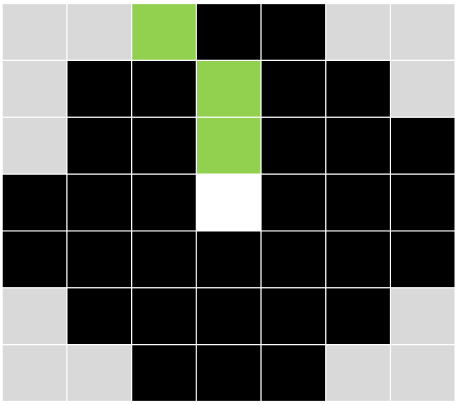
\includegraphics[width=.50\textwidth,scale=.50]{images/board}
	\caption{Diagram of an European Peg Solitaire Board Where the
				Black Squares Represent Peg Positions,
				Green Are Terminal Positions,
				Grey Are Not Positions and
				White is the Central Pixel.
			}
\end{figure}


% cite the wayback machine??
\noindent The backtracking algorithm is similar to a brute force approach to finding solutions to problems but is more systematic. It attempts to follow a logical series of decisions in solving these problems and when a block state occurs the algorithm will backtrack to previous decisions and choose different paths until a terminal (complete) state is reached. The full set of solutions to a problem can be found by continuing to run the algorithm until all paths have been searched but that is not always necessary.

\subsection{Recursive Algorithm}
\begin{figure}[H]
	\centering
	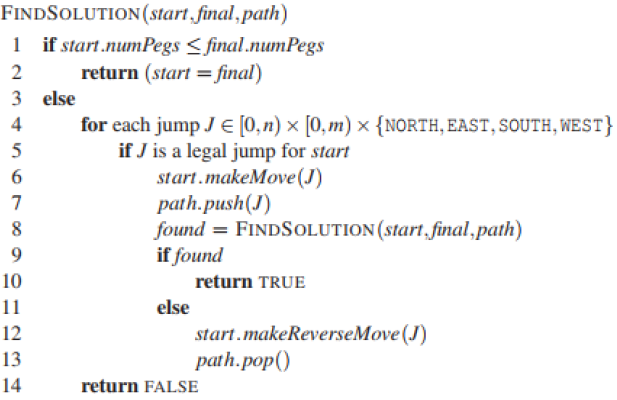
\includegraphics[width=.50\textwidth,scale=.50]{images/recursive_algorithm}
	\caption{Recursive Algorithm \cite{lab5}}
\end{figure}

\subsection{Stack Based Algorithm}

\section{Implementation}
% Comment: Talk about OpenMP, Assumptions any special things ...
% What data structures we used
% Commandline options
% how to build
% how we genereated random states rather than use a database etc...
% what random generator
% terminating conditions
% etc...


\section{Theoretical Analysis}

\section{Results}

\section{Empirical Analysis}


\section{Conclusion}

\section{Group Member Contribution}
\begin{table}[H]
\centering
\label{contribution}
\begin{tabular}{|l|l|l|}
\hline
\textbf{Member}         & \textbf{Evan Bancroft 879192} & \textbf{Jason Chalom 711985} \\ \hline
Game                    & \%                          & \%                         \\ \hline
Back Tracking Algorithm & \%                          & \%                         \\ \hline
Complexity Analysis     &                               &                              \\ \hline
Report                  &                               &                              \\ \hline
\end{tabular}
\caption{Contributions of Group Members By Task}
\end{table}

\section*{Acknowledgements}
All drawn diagrams were drawn using \url{http://draw.io/} and charts were made with Libre Office.\\ 
All the programming was done in c++ using OpenMP for its timing functions.\\


\bibliographystyle{plain}
\bibliography{biblio}{}

\end{document}